\documentclass{article}
\usepackage[utf8]{inputenc}

\title{SURP Computing Project}
\author{Simon Smith \\ Supervisor: Dr. Rachel Freisen}
\date{May 2020}


\usepackage{natbib}
\usepackage{graphicx}
\usepackage{caption}
\usepackage{subcaption}
\usepackage{indentfirst}
\usepackage{float}
\usepackage{listings}
\usepackage{amsmath}
\usepackage{geometry}
\usepackage{url}
\usepackage{textcomp}
\usepackage{titling}
\usepackage{dirtytalk}
\usepackage{gensymb}


\geometry{margin=1in}
\setlength{\parskip}{1em}
\setlength{\parindent}{3em}


\begin{document}

\maketitle

\begin{abstract}
    The following will be a brief analysis of the HC$_5$N J = 9 - 8 emission line in the HC2 of the Taurus molecular gas cloud. Some statistics, including spectral moments maps and noise reduction, will be presented.
\end{abstract}

\section{Statistics of Data Cubes}

The data cube measures the Right Ascension (RA) in the x-axis and Declination (DEC) in the y-axis, both considered in degrees. Along the z-axis, the line-of-sight frequency (or conversely, the velocity) is expressed in Hz. The map covers 0.8065$\degree$ (or 48.39') of RA and 1.2807$\degree$ (or 76.84') of DEC. In terms of pixels, the dimensions are 330 x 524, or 172920 pix$^2$. This gives an angular resolution of 8.799". Assuming that HC2 lies 140 pc away from earth, we find the spatial dimensions of the cube to be 1.97 x 3.12 pc or 406500 x 645490 AU with the resolution of each pixel being 0.00597 pc, or 1231.85 AU. The third axis shows the velocity-induced shift in the frequency of the emission line. Using the conversion equation for radio-length light, we find the resolution between subsequent layers of the cube is 71.58 m/s.

\begin{figure*}[h]
    \centering
    \captionsetup{justification=centering}
    \begin{subfigure}[H]{0.4\linewidth}
        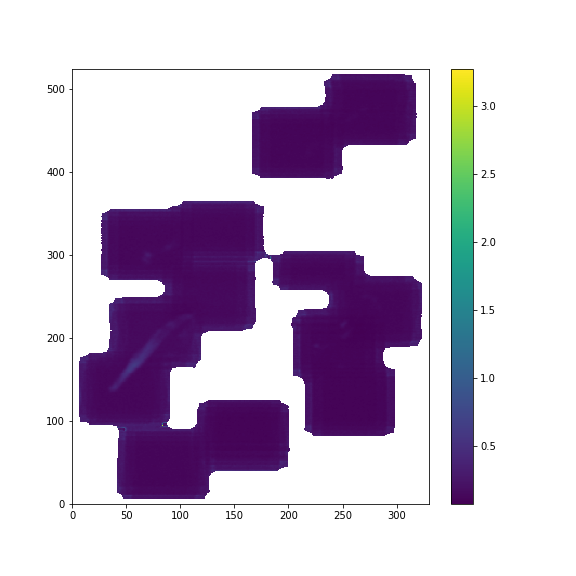
\includegraphics[width=\linewidth]{Photos/std.png}
    \end{subfigure}
    \begin{subfigure}[H]{0.4\linewidth}
        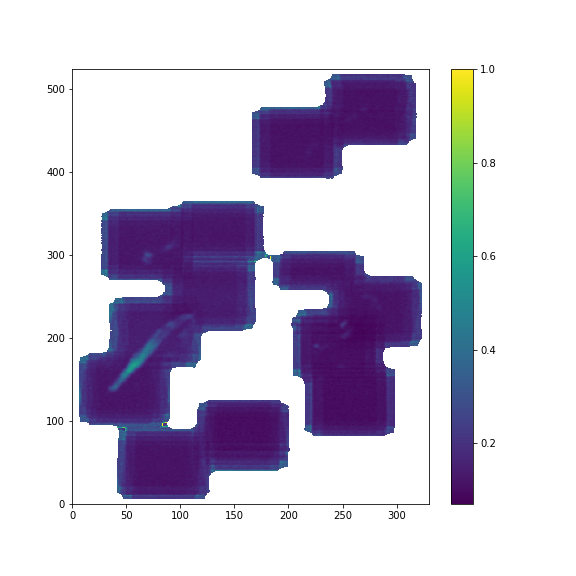
\includegraphics[width=\linewidth]{Photos/std_capped.png}
    \end{subfigure}
    \captionsetup{justification=centering,margin=1cm}
    \caption{The standard deviation of the data cube over the 0th axis (left) and the same figure but with a maximum value of unity to better exhibit the structure of the map (right).}
    \label{fig:std}
\end{figure*}

From the data cube, I took the standard deviation along the 0th axis, basically collapsing along the z-axis, to retain the same x,y dimensions while getting the standard deviation of each pixel. There is some clear structure to this map, particularly where the main feature of the cloud lies on the lower left-hand side of the frame. However, there are a couple tiny regions of very high noise which over power the more subtle contours of the data, so in the second frame, I put a limit on the colorbar values, allowing it to peek through. This revealed some potential molecular cloud structure hiding in the upper left of the frame as well as some features in the middle right cube. On the right of Figure \ref{fig:std}, there are two more bars of higher noise, below the main feature and in the upper middle that don't seem cloud-like, but we shall investigate further soon enough! There also seems to be some systematic noise appearing along edges, and especially in the corners of the data squares.

To find the deviations corresponding only to the noise, I approached the problem pixel by pixel, as I couldn't figure out a simple mask that would do cover up on all the blemishes at once. The structure in the original map corresponds to regions where spectral emission dominates the noise, leading to high standard deviations. To ignore the emission, I went pixel by pixel, examining the individual spectra and identifying the peak or peaks present. Using a scipy module, I found the widths of the peaks and took a standard deviation of only the spectral data on either side of the peaks. The resulting noise map had much of the previous physical structure filtered out.

A note, I considered trying to FFT a small section of the noice to see if some frequencies could just be subtracted out as I know that's a technique used in noise reduction for audio files, but I don't have enough experience in that area to really know what I'm doing...

\begin{figure*}[h]
    \centering
    \captionsetup{justification=centering}
    \begin{subfigure}[H]{0.4\linewidth}
        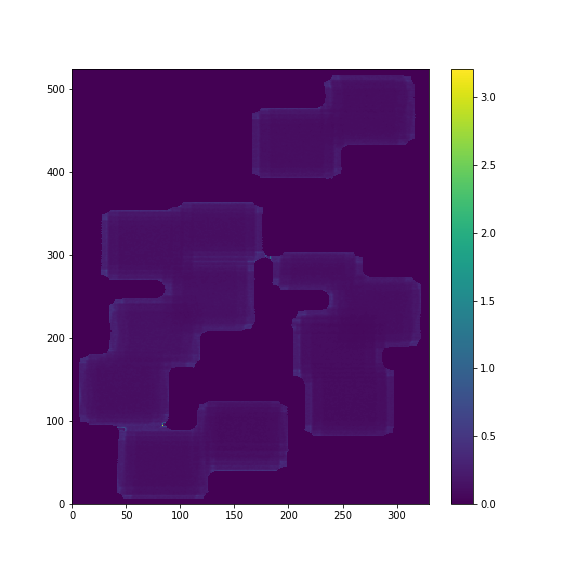
\includegraphics[width=\linewidth]{Photos/std_nn.png}
    \end{subfigure}
    \begin{subfigure}[H]{0.4\linewidth}
        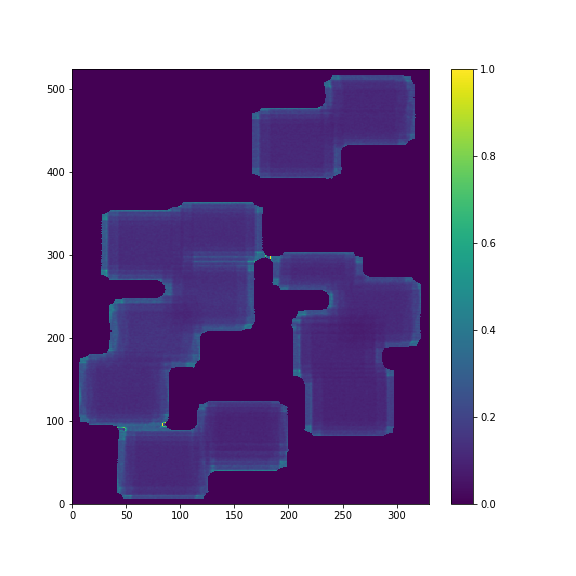
\includegraphics[width=\linewidth]{Photos/std_nn_capped.png}
    \end{subfigure}
    \captionsetup{justification=centering,margin=1cm}
    \caption{The standard deviation of the data cube without molecular cloud structure over the 0th axis (left) and the same figure but with a maximum value of unity to better exhibit the nuance of the map (right).}
    \label{fig:std_nn}
\end{figure*}

Here in Figure \ref{fig:std_nn}, the left image lacks the main molecular cloud contribution from before, but even when we move the right image, where the same intensity constraint has been applied, we see that, as expected, the two bright bars were in fact just regions of higher noise, possibly due to those being boundaries between neighbouring data cubes. This "boundary as high noise area" hypothesis is supported by the lack of structure in the right-hand figure. Those faint traces of molecular gas cloud seen in the right-hand side of Figure \ref{fig:std} are absent in this masked version.

\pagebreak

\begin{figure*}[h]
    \centering
    \captionsetup{justification=centering}
    \begin{subfigure}[H]{0.4\linewidth}
        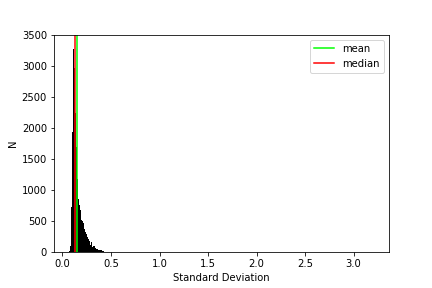
\includegraphics[width=\linewidth]{Photos/std_hist.png}
    \end{subfigure}
    \begin{subfigure}[H]{0.4\linewidth}
        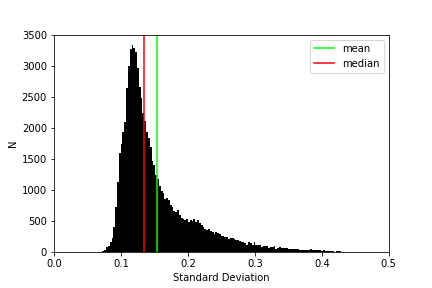
\includegraphics[width=\linewidth]{Photos/std_hist_lim.png}
    \end{subfigure}
    \captionsetup{justification=centering,margin=1cm}
    \caption{Distribution with natural bounds (left) and limited at 0.5 (right).}
    \label{fig:std_hist}
\end{figure*}

The distribution of the deviations shows what we can perceive, that most of the noise is quite small with several large outliers as seen in Figure \ref{fig:std_hist}. If we let the distribution use it's natural bounds we can assume that there are a handful of deviations around the 3 position. Limiting the bounds, we can see the shape of the distribution much better, as it rises quickly to peak around 1.2, falling away slower. The mean is 1.54 while the median is 1.34. There are far, far more data points in the main peak than there are outliers, so I took a mean of the data as if the maximum value was 0.5 and found it to differ from the true mean by parts in a thousand.

\pagebreak

\section{Moment Maps}

Maps were made of the zeroth, first, and second moments of the data cubes. Each of them had their maximum and minimum values tweaked as outliers were overpowering the contour lines of the finer details. The description of each will be described in the figure caption and the method can be found in the jupyter notebook.

\begin{figure}[H]
    \centering
    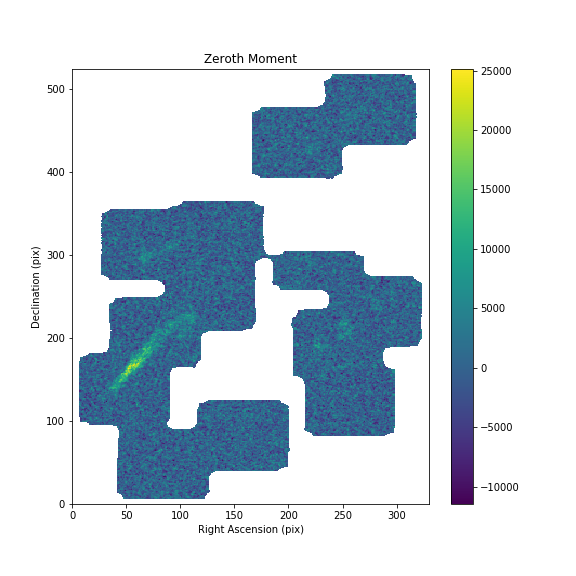
\includegraphics[width=0.8\linewidth]{Photos/M_0.png}
    \caption{The zeroth moment of the data is representative of the total intensity along each pixel. We get a fairly clean view of where molecular gas resides from the main feature in the lower left, as well as splotches in the upper left, middle right, and even hints in the upper right. The standard deviation was also divided out of this data set to help mask the effect of outliers on the clarity of the final image.}
    \label{fig:M0}
\end{figure}

\begin{figure}
    \centering
    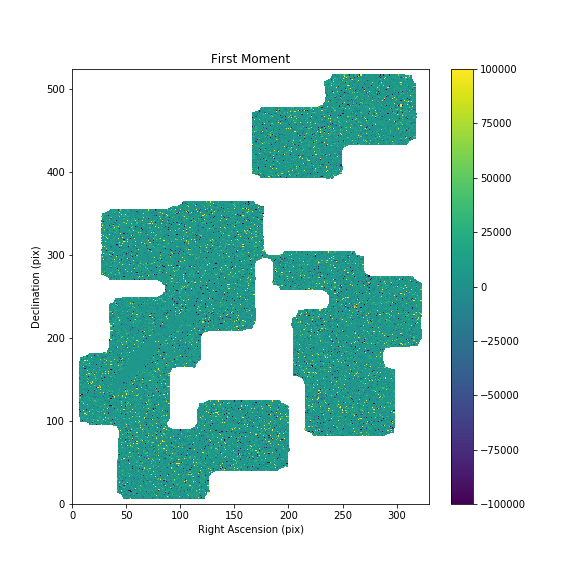
\includegraphics[width=0.8\linewidth]{Photos/M_1.png}
    \caption{The first moment interprets the average velocity of the gas along a pixel. The idea here is that if there is no structure, then the gas is moving in any given direction with a velocity related to the Maxwell speed distribution for the temperature of the gas. Hotter gas will be moving more quickly. The noise is expected where there is no structure, but in positions where we know the cloud exists, we can just see a region of turquoise, roughly elliptical in shape. The color bar tells us that this shape has an average velocity of close to zero, meaning that this clump of gas is not moving in any particular direction, as expected for a cold, dense gas cloud.}
    \label{fig:M1}
\end{figure}

\begin{figure}
    \centering
    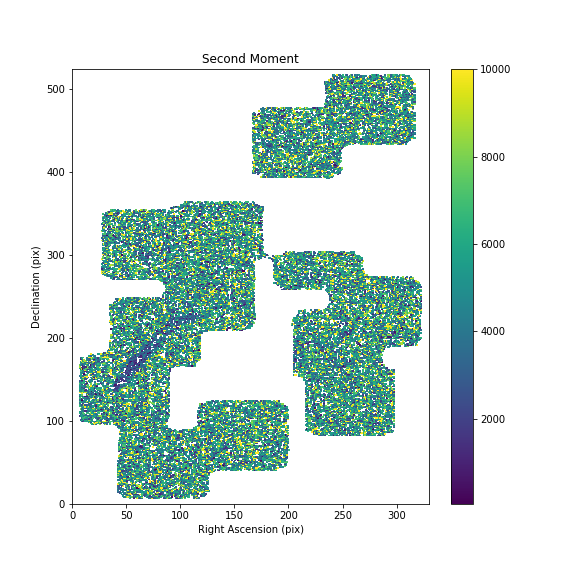
\includegraphics[width=0.8\linewidth]{Photos/M_2.png}
    \caption{The second moment of the data cube is quite interesting as it gives insight into the velocity dispersion of the gas. This relates to the thermal noise again, but rather than finding the average velocity, we learn about how much fluctuation exists amongst the entire spectrum of one pixel. Once again, we expect areas of less order and higher temperature to have higher dispersions, due to the thermal fluctuations and more random nature of the gas. We clearly see the main structure of the gas cloud, once again represented by lower values. This is because in a cold, dense gas cloud, the particles are moving more so in unison, from any currents within the gas cloud, and they also have lower chance of thermal fluctuation.}
    \label{fig:M2}
\end{figure}

\end{document}
